\section{Medical Segmentation data}
% TODO Insert Image for Dataset visualize
Due to restrictions in medical data, one of the problem we faced is finding some potentially useful segmentation dataset. We found it reasonable to start with same domain dataset so we focus the dataset on Lung CT volumes. The samples are showed using MITK workbench because it is freely available on MacOS and gives Axil Saggital and Coronal view for demonstration.
\begin{itemize}
	\item NSCLC (Non small cell Lung Cancer) Dataset consists of 402 CT scans where 78 cases has Pleural Effusion(PE). Besides the PE label, left and right lung mask is provided for segmentation training.
	\item MSD Tumor segmentation dataset consists of 63 labelled volumes non small cell lung cancer infected area. Unfortunately lung area are not labeled.
	\item Strucseg Dataset consists of 50 lung cancer patients of Lung cancer. Both organ segmentation and gross target segmentation data is annotated. However, the dataset require some documentation work and we have signed the data agreement to their email, and we cannot guarantee they will reply.
	\end{itemize}
\section{Data Processing and preprocessing}
All the dataset we have collected so far are stored as NIFTI Format. We found SimpleITK\footnote{https://simpleitk.org/} is widely used in the medical application. The data was read in as itk image with SimpleITK tool. Figure \ref{fig:original} and \ref{fig:padded} showes the original and padded volumes.
\subsubsection*{Padding}
We decided to train a 3D network as baseline and the COVID-19 Lung scan we have are in different shape. Specifically 10 higher resolution images with 512 * 512 * 134 and 10 lower resolution images with 630 * 630 * 14. And usually medical data volume is not usually a cube, we first implemented a network that can pad any volume with edge padding into a desirable shape.
%TODO insert image here
\begin{figure}
\centering
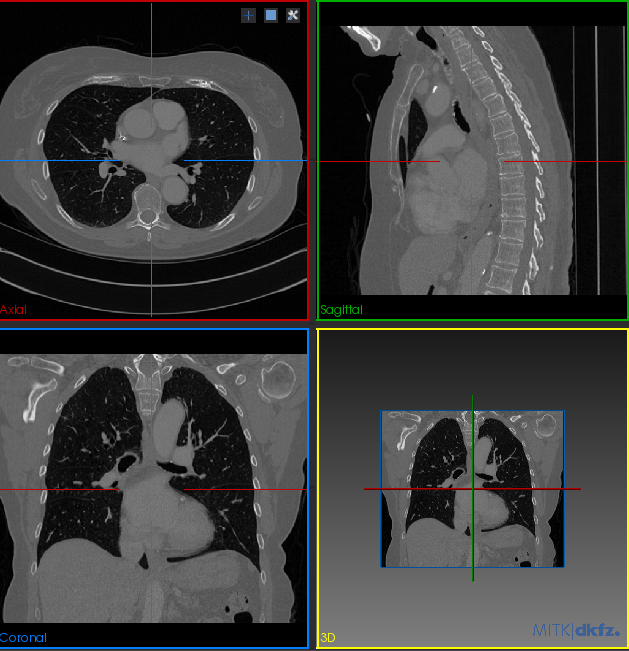
\includegraphics[width = 0.8\textwidth]{img/Original_ct.png}
\caption{Original CT image}
\label{fig:original}
\end{figure}

\begin{figure}
\centering
\includegraphics[width = 0.8\textwidth]{img/Padded_CT.png}
\caption{Padded CT into Cube}
\label{fig:padded}
\end{figure}

\subsubsection*{Augmentation through physical transformation}
Follow the suggestion in paper \cite{zhang_when_2019}, we performed augmentation on 3D images using the physical transformation such as random scale rotation. We are still improving our eclastic transformation. Figure \ref{fig:rotation} and \ref{fig:eclastic} shows the original and padded volumes.
\begin{figure}
\centering
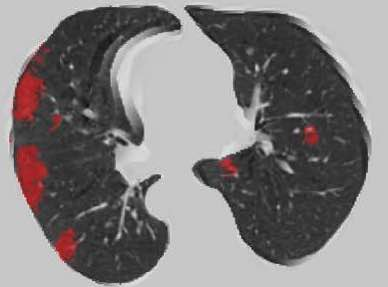
\includegraphics[width = 0.8\textwidth]{img/rotation.png}
\caption{An example Rotation}
\label{fig:rotation}
\end{figure}

\begin{figure}
\centering
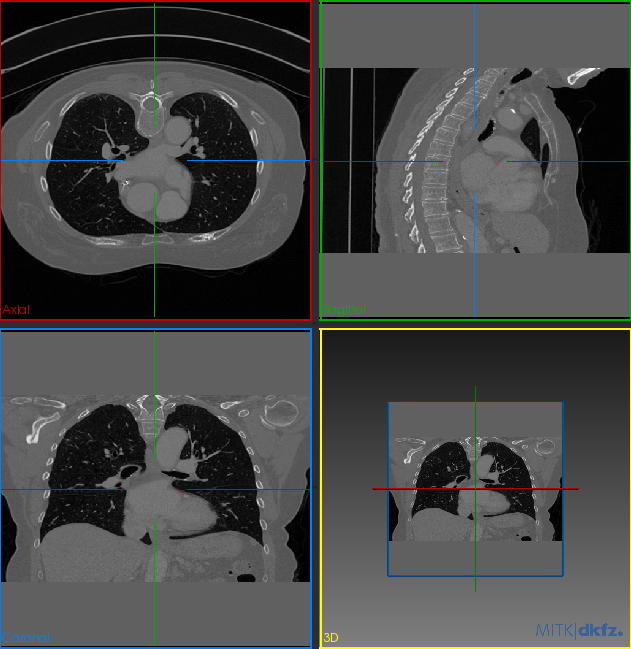
\includegraphics[width = 0.8\textwidth]{img/eclastic.png}
\caption{Eclastic transformation}
\label{fig:eclastic}
\end{figure}

\section{Brief plan}
Based on the current background review, we group the project into three Large categories: Augmentation, Model and Evaluation(CAM as extension). Here we sketch a brief plan of the project that each block has a planned implementation and potential extension.


\begin{table}[]
\begin{tabular}{lll}
\hline
\hline
Task                       & Subtask                  & Time (week commencing)       \\
\hline
Augmentation               & Traditional Aug          & June $6^{th}$                \\
Augment extension          & Mixup based              & --                           \\
Augment extension          & Learning based           & --                           \\
Across disease Transfer    & Basic 3D implementation  & June $15^{th}$               \\
                           & Freezing layers          & June $22^{th}$               \\
                           & Transfer experiment      & June $29^{th}$               \\
Extension Model            & Few shot learning design & July $6^{th}$                \\
                           & implementation           & No later than July $13^{th}$ \\
                           & Experiment               & --                           \\
Explainability (Extension) & CAM reading              & --                           \\
                           & Implementation           & --                  			 \\
\hline    
\hline    
\end{tabular}
\caption{Brief Project Plan}
\label{tab:Projplan}
\end{table}